\documentclass[12pt, t]{beamer}
\usepackage{graphicx}
\usepackage{amsmath}
\usepackage{setspace}
\usepackage{float} 
\usepackage{multido}
\usepackage{multirow}
\usepackage{array}
\usepackage{enumerate}
\usepackage{booktabs}
\usepackage{indentfirst} 
\usepackage[style=mla]{biblatex}
\usepackage{subcaption}
\usepackage{hyperref}
\usepackage{textpos}

\makeatletter
\let\@@magyar@captionfix\relax
\makeatother

\definecolor{Turquoise3}{RGB}{0, 134, 139}
\renewcommand{\emph}[1]{{\color{Turquoise3}\textsl{#1}}}
\newcommand{\C}{\mathbb{C}} \newcommand{\F}{\mathbb{F}} \newcommand{\R}{\mathbb{R}} \newcommand{\Q}{\mathbb{Q}}
\newcommand{\N}{\mathbb{N}}
\newcommand{\myseries}[2]{$#1_1,#1_2,\dots,#1_#2$}
\newcommand{\nullspace}{~\\[15pt]}
\newcommand{\remark}{\textbf{Remark: }}
\newcommand{\scp}[2]{\langle\,#1\,,\,#2\,\rangle} \newcommand{\scpp}{\langle\,\cdot\,,\,\cdot\,\rangle}


\usetheme{Madrid}
\setbeamertemplate{navigation symbols}{}

\addtobeamertemplate{frametitle}{}{
\begin{textblock*}{100mm}(0.85\textwidth,-1cm)

\includegraphics[height=1cm]{Figures/logo/logo.png}
\end{textblock*}}

\definecolor{themecolor}{RGB}{25,25,112} 

\usecolortheme[named=themecolor]{structure}

\setbeamertemplate{items}[default]

\hypersetup{
    colorlinks=true,
    linkcolor=themecolor,
    filecolor=themecolor,      
    urlcolor=themecolor,
    citecolor=themecolor,
}

\title{VV186 RC Part I}
\subtitle{\textbf{Logic}\\``Without logic, mathematics will falls apart... "}
\institute[UM-SJTU JI]{University of Michigan-Shanghai Jiao Tong University Joint Institute}
\author{Pingbang Hu}

\begin{document}

\begin{frame}
    \titlepage
    \begin{center}
        
\includegraphics[height=2cm]{Figures/logo/logo2.png}
    \end{center}
\end{frame}

\begin{frame}
    \
    \frametitle{Course Description}
    \begin{itemize}
        \item What do Vv186-Vv285-Vv286 course series teach in general?
        \item What are the difference between Vv186 and high school math?
        \item How to learn well in Vv186?
    \end{itemize}
\end{frame}

\begin{frame}
    \frametitle{How to study Vv186 well?}
    \begin{itemize}
        \item Preview and review course materials. Please always DO refer to Horst's slides.
        \item Concept is important. There will be concept checking paper available.
        \item Do assignments by your own.
        \item Don't do Too Much math exercise!
        \item Leave at least half a week to prepare for Vv186 exams.
    \end{itemize}
\end{frame}

\begin{frame}
    \frametitle{Pay attention to following...}
    For Vv186 series...
    \begin{itemize}
        \item \textbf{Forget EVERYTHING you have learned in school before.}
    \end{itemize}

    For this RC class section...
    \begin{itemize}
        \item Do think more about the question in ``()''. \\e.g. ``(How to prove?)''
        \item You are welcome to ask questions in an adequate manner.
        \item The class is designed to be interactive. Don't be so shy!
        \item Focus more on the idea of a proof. Don't just "recite" everything.
    \end{itemize}
\end{frame}

\begin{frame}
    \
    \frametitle{Overview}
    \begin{enumerate}
        \item Notation
        \item Statement
        \item Logical Operation
        \item Truth Table
        \item Relations between Statements
        \item Logical Quantifiers
        \item Sets
        \item Set Operations
        \item Ordered Pairs
        \item Russel Antinomy
        \item Exercises
    \end{enumerate}
\end{frame}

\section{Notation}
\begin{frame}
    \frametitle{Notation}
    Just one thing you need to pay attention to.\\
    
    \begin{center}
        \textbf{Always refer to Horst's convention.}
    \end{center}
    
\end{frame}

\subsection{Statement}
\begin{frame}
    \frametitle{Statement}
    \begin{itemize}
        \item True statement
        \item False statement
        \item \emph{Vacuous Truth}
        \item Statement variable
        \item Statement structure \\
            e.g. quantifier, predicate, specific value
    \end{itemize}
\end{frame}

\subsection{Logical Operation }
\begin{frame}
    \frametitle{Logical Operation}
\vspace{1.5cm}
    \begin{table}
        \centering
        \resizebox{6cm}{!}{%
        \begin{tabular}{cccc}
            \toprule
            \multicolumn{4}{c}{Logical Operation}\\
            \midrule
            $\neg$ & &Negation\\
            $\wedge$ & &Conjunction \\
            $\vee$ & &Disjunction\\
            \bottomrule
        \end{tabular}%
        }
    \end{table}
    
\end{frame}

\subsection{Truth Table}
\begin{frame}
    \frametitle{Truth Table}
    How to use Truth Table?
    \begin{itemize}
        \item Understand what the problem is about.
        \item Set up a Truth Table.
        \item Always cover all possible cases.
    \end{itemize}
Just to show you how powerful the concept of Truth Table is, here is an example.
\end{frame}

\subsection{Example of real engineering application}
\begin{frame}
    \frametitle{Application of Truth Table}
Have you ever consider how a computer add two number?\\
A: It is implemented by logic gates, and then circuits.\\
Introduce some logic gates.
\begin{figure}
    \centering
    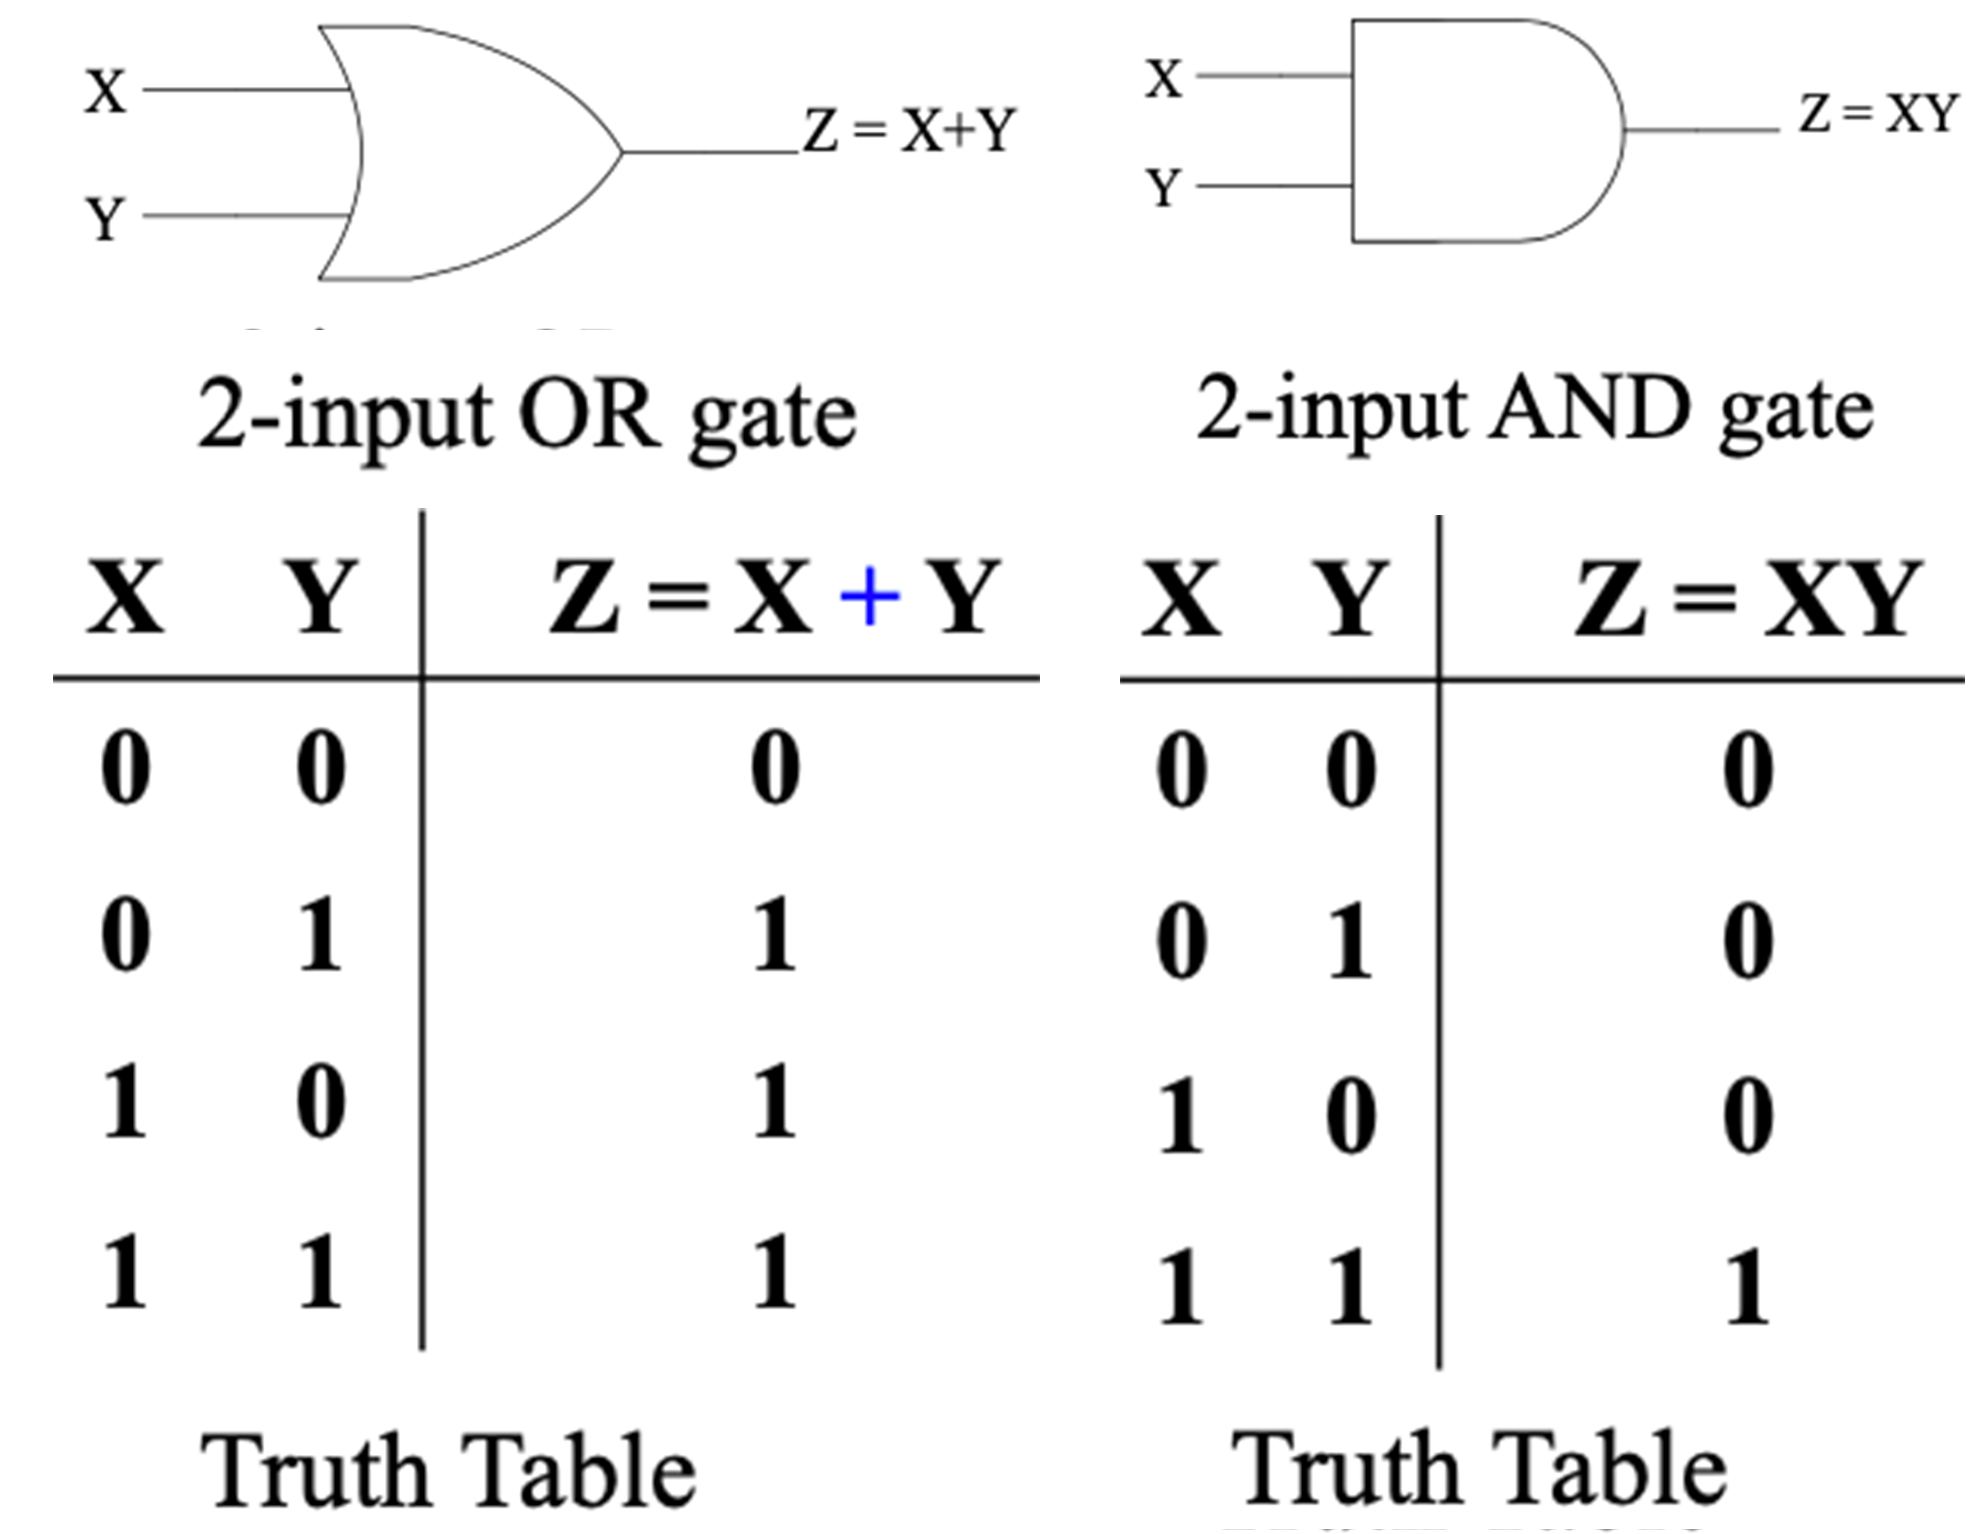
\includegraphics[width=7cm]{Figures/Logic.png}
\end{figure}
\end{frame}


\begin{frame}
    \frametitle{Adder}
Then, we can consider following:\\
\begin{center}
    \textbf{Given two numbers as input, how to add them together?}\\
\end{center}

As we all know, circuits work with binary number, e.g. 01011...\\
So, the question becomes
\begin{center}
    \textbf{How to add two one digit binary numbers?}\\
\end{center}

The idea is quite simple, that is let the circuit \emph{mimic} the action when we perform addition.
In other words, we want this circuit to cover all possible cases when we do the basic addition, namely\\
\begin{align*}
   00+00=00 \quad 00+01=01 \quad 01+00=01 \quad 01+01=10 
\end{align*}
\end{frame}    

\begin{frame}
    \frametitle{Adder}
We consider how each result's digit will react to the changing of input by constructing a Truth Table as follows:
\begin{figure}
    \centering
    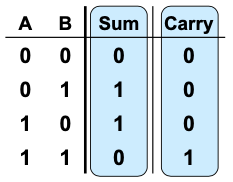
\includegraphics[width=5cm]{Figures/Adder_T.png}
\end{figure}
Then if you done your assignment 1.4, you should know you can construct a \emph{logic equation} from this Truth Table for \textbf{Sum} and \textbf{Carry}.\\
\end{frame}   


\begin{frame}
    \frametitle{Logic gates for Adder}    
\begin{align*}
    Sum=A'B+AB' \quad Carry=AB
\end{align*}
Then we can get following circuit
\begin{figure}
    \centering
    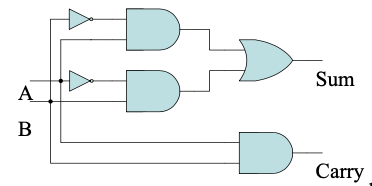
\includegraphics[width=5cm]{Figures/HalfAdder.png}
\end{figure}
Which is so-called \emph{Half Adder}.
\end{frame}

\begin{frame}
    \frametitle{More about Adder \dots}    
You can design a more complicated circuit by using same method, like:
\begin{figure}
    \centering
    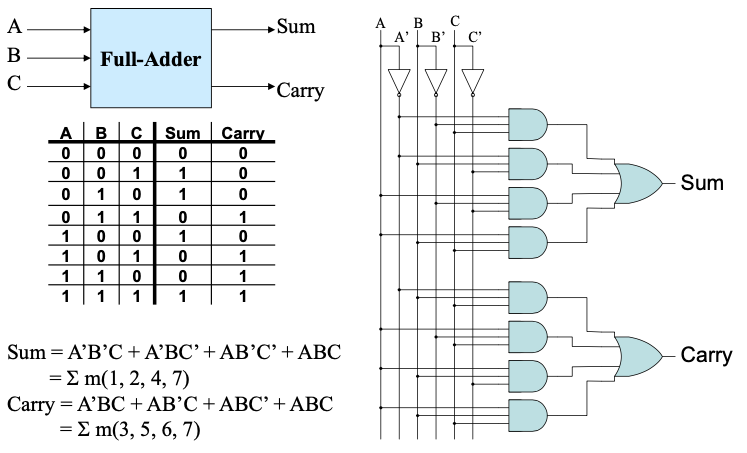
\includegraphics[width=9cm]{Figures/FullAdder.png}
\end{figure}
Which is so-called \emph{Full Adder}. You will learn these interesting concept in VE270.
\end{frame}

\begin{frame}
    \frametitle{Relations between Statements}
    \begin{itemize}
        \item Implication
        \begin{equation*}
            A \Rightarrow B
        \end{equation*}
        \item Equivalence
        \begin{equation*}
            A \Leftrightarrow B
        \end{equation*}
        \item Contraposition
        \begin{equation*}
            (A\Rightarrow B) \Leftrightarrow (\neg A \Leftarrow \neg B)
        \end{equation*}
    \end{itemize}
Proof of the contraposition (\textbf{de Morgan rules}):
    \begin{figure}
        \centering
        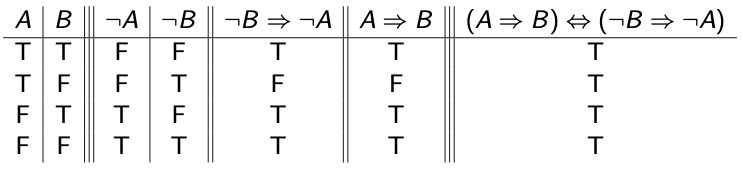
\includegraphics[width=10cm]{Figures/TruthTable.png}
    \end{figure}
And this is the concept of \emph{tautology}
\end{frame}


\begin{frame}
    \frametitle{Exercise}
    Let $P,Q$ be two sets such that $P \subseteq Q$. Then what is the relation between these
    two statements?
    \\ \center Statement A: $x \in P$. Statement B: $x \in Q$.

\end{frame}

\begin{frame}
    \frametitle{Logical Quantifiers}
    \begin{table}
        \centering
        \resizebox{12cm}{!}{%
        \begin{tabular}{ccc}
            \toprule
            \multicolumn{3}{c}{Logical Quantifiers}\\
            \midrule
            Sign & Type & Interpretation\\
            \hline
            $\forall$ & universal & for any; for all\\
            $\exists$ & existential & there exist; there is some\\
            $\forall \dots \forall \dots $ & nesting quantifier& for all \dots for all \dots \\
            $\exists \dots \exists \dots $ & nesting quantifier& there exists \dots (such that) there exist \dots \\
            .&.&.\\
            .&.&.\\
            .&.&.\\
            \bottomrule
        \end{tabular}%
        }
    \end{table} 
\end{frame}

\begin{frame}
    \frametitle{Sets}
\begin{enumerate}
    \item What is a set?
    \item Common set types
    \begin{itemize}
        \item Empty set: $\emptyset := \{x:x\neq x\}$
        \item Total set
        \item Subset
        \item Proper subset
        \item Power set
    \end {itemize}

\end{enumerate}

\par Simple question:
\center Why is $\emptyset$ a subset for any set $X$?
\end{frame}

\begin{frame}
    \frametitle{Example}
let $A:= \{4,5,6\}$ be a set.
\begin{itemize}
    \item The total set can be $\mathbb{N}$
    \item $B:= \{4,5,5,6,6\}=A$
    \item $C=\{1,5\}\subseteq A$
    \item $P:=\{\emptyset,\{4\},\{5\},\{6\},\{4,5\},\{5,6\},\{4,6\},\{4,5,6\}\}$ 
    \\\hspace{1em} is the power set of $A$. (What is the cardinality of $A$ ?)
\end{itemize}
\end{frame}

\begin{frame}
    \frametitle{Set Operations}
Define 
\begin{equation*}
    A:=\{1,2\} \quad B:=\{2,3\} \quad M:=\{1,2,3,4,5\}
\end{equation*}
\begin{table}
    \centering
    \resizebox{6cm}{!}{%
    \begin{tabular}{ccc}
        \toprule
        \multicolumn{3}{c}{Set Operations}\\
        \midrule
        $A\cup B$ & Union & $\{1,2,3\}$\\
        $A\cap B$ & Intersection & $\{2\}$\\
        $A\setminus B$ & Difference & $\{1\}$\\
        $A^c $ & Complement & $\{3,4,5\}$\\
        \bottomrule
    \end{tabular}%
    }
\end{table}  

\par Simple question:
\center What is $M^c$ ? Also, what is $\emptyset^c$ ?
\end{frame}

\begin{frame}
    \frametitle{Ordered Pairs}
\begin{itemize}
    \item What is an ordered pair?
    \item What is the difference between ordered pair and set?
    \item Concept of \emph{Cartesian product}.
\end{itemize}
\end{frame}

\begin{frame}
    \frametitle{Russel Antinomy}
There exist several paradox in native set theorey, including:\\
\begin{enumerate}
    \item Russel Antinomy
    \item Cantor's paradox
    \item Burali-Forti paradox
\end{enumerate}
\par \hspace{1em} The above paradoxes illustrate the fundemental flaw of our naive theorey, namely
it's not \textbf{well-defined}.\\
\par \hspace{1em} However, these problem can be solved if we replaced naive set theorey by a 
\emph{modern axiomatic set theory}, but the detail about it is beyond our scope.\\
\end{frame}

\begin{frame}
    \frametitle{Exercises}
1. Let $A, B, C$ be three statements. Use truth table to prove that 
\begin{equation*}
    (A\vee B)\wedge C \equiv (A\wedge C)\vee (B\wedge C)
\end{equation*}
\end{frame}

\begin{frame}
    \frametitle{Exercises}
2. Let $A, B, C$ be three sets. Prove that
\begin{equation*}
    (A\cup B)\cap C =(A\cap C)\cup (B\cap C)
\end{equation*}
From Exercise 1 \& 2, we can see that sets and statements are similar.
\end{frame}

\begin{frame}
    \frametitle{Exercises}
3. Check whether the following sentences are true statement, false statement, or not a statement.
\begin{itemize}
    \item $\forall x, y\in \mathbb{R}, x^2+y^3\geq 0$
    \item Let  $f(a)=a^4$, then $f(0)>0$
    \item For any $a\in \mathbb{R}, a^4>0$
    \item An African Elephant is very big.
    \item Let $A, B$ be two statements, then $(A\vee B)\Leftrightarrow\neg(\neg A\wedge\neg B)$
\end{itemize}
Simple question
\begin{center}
    Rewrite above sentences in quantifiers form if they are statement.
\end{center}

\end{frame}

\begin{frame}
    \frametitle{Exercises}
4. Use quantifiers to rewrite the following definition of covergence:
\par \vspace{2em} \hspace{1em} Let $(a_n)_{n\in \mathbb{N}}$ be a real sequence. If for some fixed $c \in \mathbb{R}$, 
for any $a>0$, there is an $N\in \mathbb{N}$, such that for all $n>N$, $|a_n-c|<a$,\\ then we
say $(a_n)$ converges.
\end{frame}

\begin{frame}
    \frametitle{Reference}
Reference.
    \begin{itemize}
        \item Exercises from 2019--Vv186 TA-Zhang Leyang.
        \item Figure for circuits from Ve270 T2-Logic Gate Slides.
    \end{itemize}
\end{frame}

\begin{frame}
    \frametitle{End}
    \vspace{2cm}
    \Huge \center  Have Fun and Learn Well!
\end{frame}


\end{document}